%%%%%%%%%%%%%%%%%%%%%%%%%%%%%%%%%%%%%%%%%%%%%%%%%%%%%%%%%%%%%%%%%%%%%%%%
%                                                                      %
%     File: Thesis_Modeling.tex                                        %
%     Tex Master: Thesis.tex                                           %
%                                                                      %
%     Author: Andre C. Marta                                           %
%     Last modified :  25 Jul 2026                                     %
%                                                                      %
%%%%%%%%%%%%%%%%%%%%%%%%%%%%%%%%%%%%%%%%%%%%%%%%%%%%%%%%%%%%%%%%%%%%%%%%

% ==============================================================================
% CHAPTER 3: SYSTEM MODELING
% ==============================================================================
\chapter{System modeling}
\label{chapter:modeling}

Real-time control needs models that are simple enough to compute quickly, yet detailed enough to capture how each vehicle actually moves and interacts with the other. The kinematics, dynamics, and physical coupling between the two vehicles let the controller predict how the system evolves and compute feasible, optimal trajectories.

The reference frames and notation are fixed first, followed by the kinematic and dynamic models of the \gls{usv} and the \gls{uav}.


% ==============================================================================
% SECTION 3.1: Reference Coordinate Frames and Notation
% ==============================================================================
\section{Reference Coordinate Frames and Notation}
\label{sec:mod_coordinates}

Deriving the equations of motion requires specifying the frames against which positions, orientations, and velocities are measured. Since the vessel and the drone move both with respect to the world and with respect to each other, a common frame of reference is required to describe their motion. Figure~\ref{fig:coordinate_frames} illustrates these frames.

\paragraph{Inertial Reference Frame $\{\mathcal{I}\}$}
This frame establishes the global coordinate system following the East-North-Up (ENU) convention, aligned with the standard ROS convention. Its origin $\mathcal{O}_I$ is fixed at an arbitrary point on the water surface within the operating area, following the usual flat-Earth convention. The axis $\mathbf{x}^{\mathcal{I}}$ points East, $\mathbf{y}^{\mathcal{I}}$ points North, and $\mathbf{z}^{\mathcal{I}}$ points upward, opposite to gravity.

\paragraph{USV Body-Fixed Reference Frame $\{\mathcal{B}_v\}$}
This frame is rigidly attached to the vessel, with origin $\mathcal{O}_v$ at its centre of gravity. This choice decouples the linear and rotational momentum equations. The forward-pointing axis $\mathbf{x}^{\mathcal{B}_v}$ defines surge, $\mathbf{y}^{\mathcal{B}_v}$ points to port (sway), and $\mathbf{z}^{\mathcal{B}_v}$ points upward (heave).

\paragraph{UAV Body-Fixed Reference Frame $\{\mathcal{B}_a\}$}
Similarly, this frame attaches to the UAV, with origin $\mathcal{O}_a$ at its centre of gravity, decoupling the translational and rotational dynamics in the same way. The longitudinal axis $\mathbf{x}^{\mathcal{B}_a}$ points forward, the lateral axis $\mathbf{y}^{\mathcal{B}_a}$ points to the left, and the vertical axis $\mathbf{z}^{\mathcal{B}_a}$ points upward, aligning with the collective thrust direction.

\begin{figure}[H]
    \centering
    % Colors: Okabe-Ito colorblind-safe qualitative palette (Okabe and Ito, 2008)
    \definecolor{okiBlue}{rgb}{0.0,0.447,0.698}       % Inertial frame {I}
    \definecolor{okiGreen}{rgb}{0.0,0.620,0.451}      % USV body frame {Bv}
    \definecolor{okiOrange}{rgb}{0.902,0.624,0.0}     % UAV body frame {Ba}
    \definecolor{okiVermillion}{rgb}{0.835,0.369,0.0} % Anchor / coupling point
    
    \begin{tikzpicture}[
        >=stealth,
        scale=1.0,
        axis/.style={->,okiBlue,thick,line width=1.2pt},
        bodyaxis/.style={->,okiGreen,thick,line width=1.2pt},
        uavaxis/.style={->,okiOrange,thick,line width=1.2pt},
        label/.style={black,font=\small},
        tether/.style={draw,line width=1.5pt,darkgray,smooth}
    ]
        % -- WATER SURFACE (z = 0) --
        \draw[black, dashed, line width=0.8pt] (-1.0,0) -- (10.0,0) node[right, font=\scriptsize, black!80] {Water Surface ($z^{\mathcal{I}}=0$)};

        % -- INERTIAL FRAME {I} --
        \coordinate (OI) at (0,0);
        \draw[axis] (OI) -- (2.0,0) node[below right,label,okiBlue] {$\mathbf{x}^{\mathcal{I}}$ (East)};
        \draw[axis] (OI) -- (1.0,0.8) node[above right,label,okiBlue] {$\mathbf{y}^{\mathcal{I}}$ (North)};
        \draw[axis] (OI) -- (0,2.0) node[above,label,okiBlue] {$\mathbf{z}^{\mathcal{I}}$ (Up)};
        \node[below left,label,okiBlue] at (OI) {$\{\mathcal{I}\}$};

        % -- USV FRAME {Bv} (Catamaran seen from the side, sitting at z=0) --
        \coordinate (Ov) at (5.5,0.45);
        \begin{scope}[shift={(Ov)}]
            % WAM-V pontoon (hull), side view
            \draw[thick,fill=gray!30] (-1.2,-0.45) -- (0.8,-0.45) to[out=0,in=-120] (1.3,-0.15) -- (-1.2,-0.15) -- cycle;
            % Support arch legs
            \draw[line width=1.5pt,black] (-0.6,-0.15) -- (-0.3,0.3);
            \draw[line width=1.5pt,black] (0.6,-0.15) -- (0.3,0.3);
            % Upper deck
            \draw[thick,fill=gray!50] (-0.5,0.3) rectangle (0.5,0.45);
            
            % Boat body axes (side/3D view)
            \draw[bodyaxis] (0,0) -- (1.8,0) node[right,label,okiGreen] {$\mathbf{x}^{\mathcal{B}_v}$};
            \draw[bodyaxis] (0,0) -- (0,1.5) node[right,label,okiGreen,xshift=2pt,yshift=-4pt] {$\mathbf{z}^{\mathcal{B}_v}$};
            \draw[bodyaxis] (0,0) -- (0.6,0.48) node[above,label,okiGreen,xshift=-3pt] {$\mathbf{y}^{\mathcal{B}_v}$};
            
            % Anchor point, vertically aligned with the CG
            \coordinate (Pa) at (0,0.45);
            \fill[white] (Pa) circle (4pt); % break the z_v arrow shaft behind the marker
            \fill[okiVermillion] (Pa) circle (2.5pt) node[above left,font=\scriptsize,black] {Anchor};
        \end{scope}

        \node[below,label,okiGreen] at ($(Ov)+(0,-0.45)$) {$\{\mathcal{B}_v\}$};

        % -- UAV FRAME {Ba} (Drone seen from the side/front, flying in 3D with pitch tilt) --
        \coordinate (Oa) at (9.0,3.5);
        \begin{scope}[shift={(Oa)}, rotate=-15]
            % Drone cross arms in 3D (side/isometric perspective)
            \draw[thick,line width=1.5pt,black] (-0.6,-0.15) -- (0.6,0.15);
            \draw[thick,line width=1.5pt,black] (-0.5,0.15) -- (0.5,-0.15);
            % Central body
            \fill[black] (0,0) circle (3.5pt);
            % The 4 rotors/propellers at the arm tips
            \draw[gray, thin] (-0.6,-0.1) ellipse (3pt and 0.8pt);
            \draw[gray, thin] (0.6,0.2) ellipse (3pt and 0.8pt);
            \draw[gray, thin] (-0.5,0.2) ellipse (3pt and 0.8pt);
            \draw[gray, thin] (0.5,-0.1) ellipse (3pt and 0.8pt);
            
            % Drone body axes (tilt with the vehicle body)
            \draw[uavaxis] (0,0) -- (1.4,0) node[right,label,okiOrange] {$\mathbf{x}^{\mathcal{B}_a}$};
            \draw[uavaxis] (0,0) -- (0,1.4) node[above,label,okiOrange] {$\mathbf{z}^{\mathcal{B}_a}$};
            \draw[uavaxis] (0,0) -- (0.5,0.4) node[above right,label,okiOrange] {$\mathbf{y}^{\mathcal{B}_a}$};
        \end{scope}
        
        \node[below,label,okiOrange] at ($(Oa)+(0,-0.50)$) {$\{\mathcal{B}_a\}$};

        % -- TETHER --
        % Smooth curve representing the tether, labeled below right to avoid overlaps with the axes
        \draw[tether] (Pa) .. controls ($(Pa)+(1.5,-0.2)$) and ($(Oa)+(-1.0,-1.0)$) .. (Oa);
        \path (Pa) .. controls ($(Pa)+(1.5,-0.2)$) and ($(Oa)+(-1.0,-1.0)$) .. (Oa);

    \end{tikzpicture}
    \caption{Reference coordinate frames $\{\mathcal{I}\}$, $\{\mathcal{B}_v\}$, and $\{\mathcal{B}_a\}$.}
    \label{fig:coordinate_frames}
\end{figure}

% ==============================================================================
% SECTION 3.2: WAM-V Surface Vessel Model
% ==============================================================================
\section{WAM-V Surface Vessel Model}
\label{sec:mod_usv}

The mathematical model of the WAM-V catamaran, covering its horizontal maneuvering dynamics and thruster allocation, forms a control-oriented state-space model suitable for trajectory tracking and predictive control.

Although a rigid body moving freely in the marine environment inherently has six degrees of freedom, the WAM-V is a vessel that moves on the surface, which allows the motion to be simplified to the horizontal plane. Under this assumption, the model is reduced to three degrees of freedom.

Predicting the vessel's motion, as needed for trajectory tracking and predictive control, requires knowing how its state changes over time for a given input. This relationship is captured by the nonlinear state-space model
\begin{equation}
    \label{eq:usv_state_space_generic}
    \dot{\mathbf{x}}_v = f(\mathbf{x}_v, \mathbf{u}_v),
\end{equation}
The state vector $\mathbf{x}_v \in \mathbb{R}^6$ is given by
\begin{equation}
    \label{eq:usv_state_vector}
    \mathbf{x}_v = [x, y, \psi, u, v, r]^T,
\end{equation}
where:
\begin{itemize}
    \item $x, y$ -- position of the origin $\mathcal{O}_v$ of $\{\mathcal{B}_v\}$ relative to $\{\mathcal{I}\}$, expressed in $\{\mathcal{I}\}$;
    \item $\psi$ -- heading of $\{\mathcal{B}_v\}$ relative to $\{\mathcal{I}\}$;
    \item $u, v$ -- surge and sway linear velocities of $\{\mathcal{B}_v\}$ relative to $\{\mathcal{I}\}$, expressed in $\{\mathcal{B}_v\}$;
    \item $r$ -- angular velocity of $\{\mathcal{B}_v\}$ relative to $\{\mathcal{I}\}$, expressed in $\{\mathcal{B}_v\}$;
\end{itemize}
The control input vector $\mathbf{u}_v \in \mathbb{R}^3$ is given by
\begin{equation}
    \label{eq:usv_input_vector}
    \mathbf{u}_v = [X, Y, N]^T,
\end{equation}
where:
\begin{itemize}
    \item $X$ -- surge force generated by the propulsion system, applied to $\{\mathcal{B}_v\}$, expressed in $\{\mathcal{B}_v\}$;
    \item $Y$ -- sway force generated by the propulsion system, applied to $\{\mathcal{B}_v\}$, expressed in $\{\mathcal{B}_v\}$;
    \item $N$ -- yaw moment generated by the propulsion system, applied to $\{\mathcal{B}_v\}$, expressed in $\{\mathcal{B}_v\}$;
\end{itemize}
The vector field $f(\cdot)$ splits into a kinematic block and a dynamic block, derived in turn in the following subsections.

\subsection{Kinematic Model}
\label{subsec:mod_usv_kinematics}
The kinematics describe how the vessel's inertial position and heading evolve as a function of its body-fixed velocities, forming the first half of \eqref{eq:usv_state_space_generic}.

Let $\mathbf{p} = x\,\mathbf{x}^{\mathcal{I}} + y\,\mathbf{y}^{\mathcal{I}}$ denote the inertial position of the origin $\mathcal{O}_v$ of $\{\mathcal{B}_v\}$. Since $\mathbf{x}^{\mathcal{I}}, \mathbf{y}^{\mathcal{I}}$ are constant, differentiating yields
\begin{equation}
    \dot{\mathbf{p}} = \dot{x}\,\mathbf{x}^{\mathcal{I}} + \dot{y}\,\mathbf{y}^{\mathcal{I}},
    \label{eq:usv_pdot_inertial_def}
\end{equation}
i.e.\ $\dot{x}, \dot{y}$ are, by definition, the components of $\dot{\mathbf{p}}$ in the inertial frame.

The surge and sway velocities $u, v$ are defined in the body-fixed frame, so that
\begin{equation}
    \dot{\mathbf{p}} = u\,\mathbf{x}^{\mathcal{B}} + v\,\mathbf{y}^{\mathcal{B}},
    \label{eq:usv_pdot_body_frame}
\end{equation}
where $\mathbf{x}^{\mathcal{B}}, \mathbf{y}^{\mathcal{B}}$ denote the basis vectors of $\{\mathcal{B}_v\}$, i.e.\ $\mathbf{x}^{\mathcal{B}_v}, \mathbf{y}^{\mathcal{B}_v}$.

Since $\{\mathcal{B}_v\}$ is rotated relative to $\{\mathcal{I}\}$ by the heading angle $\psi$, the inertial unit vectors are related to the body-fixed ones by the rotation matrix $\mathbf{R}(\psi) \in SO(2)$,
\begin{equation}
    \begin{bmatrix} \mathbf{x}^{\mathcal{I}} \\ \mathbf{y}^{\mathcal{I}} \end{bmatrix} = \mathbf{R}(\psi) \begin{bmatrix} \mathbf{x}^{\mathcal{B}} \\ \mathbf{y}^{\mathcal{B}} \end{bmatrix},
    \label{eq:usv_basis_matrix}
\end{equation}
following the standard planar rotation matrix,
\begin{equation}
    \mathbf{R}(\psi) = \begin{bmatrix} \cos\psi & -\sin\psi \\ \sin\psi & \cos\psi \end{bmatrix},
    \label{eq:usv_rotation_matrix}
\end{equation}
which is equivalent to
\begin{equation}
    \mathbf{x}^{\mathcal{B}} = \cos\psi\,\mathbf{x}^{\mathcal{I}} + \sin\psi\,\mathbf{y}^{\mathcal{I}}, \qquad
    \mathbf{y}^{\mathcal{B}} = -\sin\psi\,\mathbf{x}^{\mathcal{I}} + \cos\psi\,\mathbf{y}^{\mathcal{I}}.
    \label{eq:usv_basis_change}
\end{equation}

Substituting \eqref{eq:usv_basis_change} into \eqref{eq:usv_pdot_body_frame} and grouping terms gives
\begin{equation}
    \dot{\mathbf{p}} = \underbrace{(u\cos\psi - v\sin\psi)}_{\dot{x}}\,\mathbf{x}^{\mathcal{I}} + \underbrace{(u\sin\psi + v\cos\psi)}_{\dot{y}}\,\mathbf{y}^{\mathcal{I}}.
    \label{eq:usv_pdot_expanded}
\end{equation}
Comparing with \eqref{eq:usv_pdot_inertial_def} then directly gives
\begin{equation}
    \dot{x} = u\cos\psi - v\sin\psi, \qquad \dot{y} = u\sin\psi + v\cos\psi,
\end{equation}
which is precisely
\begin{equation}
    \label{eq:usv_kinematics_planar}
    \begin{bmatrix} \dot{x} \\ \dot{y} \end{bmatrix} = \mathbf{R}(\psi)\begin{bmatrix} u \\ v \end{bmatrix}.
\end{equation}

The heading rate follows directly from the definition of the angular velocity $r$:
\begin{equation}
    \dot{\psi} = r. \label{eq:usv_psi_dot}
\end{equation}

\subsection{Dynamic Model}
\label{subsec:mod_usv_dynamics}

The dynamics describe how the vessel's body-fixed velocities evolve as a function of the applied forces and moments, forming the second half of \eqref{eq:usv_state_space_generic}.

Unlike $\mathbf{x}^{\mathcal{I}}, \mathbf{y}^{\mathcal{I}}$, the body-fixed unit vectors $\mathbf{x}^{\mathcal{B}}, \mathbf{y}^{\mathcal{B}}$ rotate with the vehicle. Differentiating \eqref{eq:usv_basis_change} and using $\dot\psi = r$ gives
\begin{equation}
    \dot{\mathbf{x}}^{\mathcal{B}} = r\,\mathbf{y}^{\mathcal{B}}, \qquad \dot{\mathbf{y}}^{\mathcal{B}} = -r\,\mathbf{x}^{\mathcal{B}}.
    \label{eq:usv_basis_dot}
\end{equation}
The inertial velocity, expressed in the body-fixed frame, is $\dot{\mathbf{p}} = u\,\mathbf{x}^{\mathcal{B}} + v\,\mathbf{y}^{\mathcal{B}}$. Differentiating once more and substituting \eqref{eq:usv_basis_dot} yields the inertial acceleration
\begin{equation}
    \ddot{\mathbf{p}} = (\dot{u} - vr)\,\mathbf{x}^{\mathcal{B}} + (\dot{v} + ur)\,\mathbf{y}^{\mathcal{B}},
    \label{eq:usv_pddot_body_frame}
\end{equation}
where the cross terms $-vr$ and $ur$ are Coriolis/centripetal terms arising because $\{\mathcal{B}_v\}$ is a rotating, non-inertial frame.

Let $F_x, F_y$ denote the resultant surge and sway forces applied at $\mathcal{O}_v$, so that $\mathbf{F} = F_x\,\mathbf{x}^{\mathcal{B}} + F_y\,\mathbf{y}^{\mathcal{B}}$. By Newton's second law, $\mathbf{F} = m\,\ddot{\mathbf{p}}$, and comparing with \eqref{eq:usv_pddot_body_frame},
\begin{equation}
    F_x = m(\dot{u} - vr), \qquad F_y = m(\dot{v} + ur).
    \label{eq:usv_newton_linear}
\end{equation}
Since the vessel's motion is planar, Euler's rotational equation about $\mathbf{z}^{\mathcal{B}}$ takes the form
\begin{equation}
    M_z = I_z\,\dot{r},
    \label{eq:usv_euler_yaw}
\end{equation}
where $M_z$ is the resultant yaw moment about $\mathcal{O}_v$ and $I_z$ the yaw moment of inertia.

The resultant force and moment $F_x, F_y, M_z$ combine two contributions: the thrust generated by the propulsion system, $X, Y, N$, and the hydrodynamic damping opposing the vessel's motion. This damping follows the standard linear-plus-quadratic model for surface vessels~\cite{fossenHandbookMarineCraft2011}. The quadratic surge term is further split into forward and backward coefficients, to capture the asymmetric drag between the two directions:
\begin{equation}
    F_x = X - \big(X_u + X_{uu}^{\pm}|u|\big)u, \qquad
    X_{uu}^{\pm} = \begin{cases} X_{uu}^{+}, & u \geq 0 \\ X_{uu}^{-}, & u < 0 \end{cases}
    \label{eq:usv_damping_surge}
\end{equation}
\begin{equation}
    F_y = Y - \big(Y_v + Y_{vv}|v|\big)v, \qquad
    M_z = N - \big(N_r + N_{rr}|r|\big)r.
    \label{eq:usv_damping_sway_yaw}
\end{equation}

Substituting \eqref{eq:usv_damping_surge}--\eqref{eq:usv_damping_sway_yaw} into \eqref{eq:usv_newton_linear} and \eqref{eq:usv_euler_yaw}, and solving for the accelerations, gives the dynamic block of \eqref{eq:usv_state_space_generic}:
\begin{equation}
    \dot{u} = \frac{1}{m}\Big[X - \big(X_u + X_{uu}^{\pm}|u|\big)u\Big] + vr,
    \label{eq:usv_udot}
\end{equation}
\begin{equation}
    \dot{v} = \frac{1}{m}\Big[Y - \big(Y_v + Y_{vv}|v|\big)v\Big] - ur,
    \label{eq:usv_vdot}
\end{equation}
\begin{equation}
    \dot{r} = \frac{1}{I_z}\Big[N - \big(N_r + N_{rr}|r|\big)r\Big].
    \label{eq:usv_rdot}
\end{equation}

\subsection{Thruster Allocation}
\label{subsec:mod_usv_thruster_allocation}

The thruster allocation maps the physical actuator commands, the left and right thrust magnitudes $T_L, T_R$ and azimuth angles $\alpha_L, \alpha_R$, to the resultant force and moment $X, Y, N$ required by the dynamics of Section~\ref{subsec:mod_usv_dynamics}, according to the geometry shown in Figure~\ref{fig:usv_planar_model}.

\begin{figure}[H]
    \centering
    % Colors: Okabe-Ito colorblind-safe qualitative palette. Body axes stay neutral
    % gray so color draws the eye to the forces, the physically meaningful content.
    \definecolor{okiBlue}{rgb}{0.0,0.447,0.698}       % Resultant control forces X, Y, N
    \definecolor{okiVermillion}{rgb}{0.835,0.369,0.0} % Raw thruster forces T_L, T_R
    
    \begin{tikzpicture}[
        >=stealth,
        scale=1.45,
        every node/.style={font=\small},
        axisV/.style={->, black!60, line width=1.3pt},
        forceVec/.style={->, okiVermillion, line width=1.4pt},
        resForce/.style={->, okiBlue, line width=1.3pt},
        dimLine/.style={<->, >=stealth, black!75, line width=0.6pt, font=\footnotesize},
        guideLine/.style={dashed, black!35, line width=0.5pt}
    ]
        % Geometrical Parameters
        \def\xarm{-2.6}
        \def\yarm{1.6}
        \def\alphaL{28}
        \def\alphaR{-22}

        % -- CATAMARAN CROSSBEAMS & DECK --
        % Connecting crossbeams between pontoons
        \draw[fill=gray!40, draw=black!70, line width=0.8pt] 
            (-1.4, -1.6) rectangle (-1.0, 1.6);
        \draw[fill=gray!40, draw=black!70, line width=0.8pt] 
            (0.6, -1.6) rectangle (1.0, 1.6);

        % Central Deck (with clean margins from pontoons)
        \draw[fill=gray!15, draw=black!65, line width=0.85pt, rounded corners=3pt] 
            (-1.5, -1.0) rectangle (1.1, 1.0);

        % Left Pontoon (Port)
        \draw[fill=gray!25, draw=black!85, line width=1.0pt, rounded corners=2pt]
            (-2.7, 1.35) -- (1.5, 1.35) -- (2.8, 1.6) -- (1.5, 1.85) -- (-2.7, 1.85) -- cycle;
        % Label shifted forward to avoid the y-axis at x=0
        \node[font=\scriptsize, black!65] at (0.8, 1.6) {Port Pontoon};

        % Right Pontoon (Starboard)
        \draw[fill=gray!25, draw=black!85, line width=1.0pt, rounded corners=2pt]
            (-2.7, -1.85) -- (1.5, -1.85) -- (2.8, -1.6) -- (1.5, -1.35) -- (-2.7, -1.35) -- cycle;
        % Label shifted forward to avoid the dimension guideline at x=0
        \node[font=\scriptsize, black!65] at (0.8, -1.6) {Starboard Pontoon};

        % Longitudinal Centerline
        \draw[guideLine] (-3.6, 0) -- (3.6, 0);

        % -- CENTER OF GRAVITY (CG) & BODY AXES --
        \fill[black] (0,0) circle (2.5pt);
        \draw[line width=0.7pt, black] (0,0) circle (5.0pt);
        \node[below left, font=\scriptsize, black, xshift=-4pt, yshift=-7pt] at (0,0) {$\mathcal{O}_v$ (CG)};

        % Body axes {Bv}
        \draw[axisV] (0,0) -- (3.6, 0) node[right, black!60] {$\mathbf{x}^{\mathcal{B}_v}$ (surge, $u$)};
        \draw[axisV] (0,0) -- (0, 2.7) node[above, black!60] {$\mathbf{y}^{\mathcal{B}_v}$ (sway, $v$)};
        
        % Yaw rate r (curved orange arrow in Quadrant I: R=0.65, 15° to 80°, span 65°)
        \draw[->, line width=1.1pt, black!60] (0.628, 0.168) arc (15:80:0.65) 
            node[above right, font=\small, black!60, xshift=-1pt, yshift=1pt] {$r$};

        % Resultant Control Forces at CG (X, Y, N) in MATLAB Blue
        \draw[resForce] (0,0) -- (1.5, 0) 
            node[above, font=\footnotesize, okiBlue, xshift=-2pt, yshift=2pt] {$X$};
        \draw[resForce] (0,0) -- (0, 1.4);
        % Y placed cleanly in the gap between deck (y=1.0) and pontoon (y=1.35)
        \node[left, font=\footnotesize, okiBlue, xshift=-2pt] at (0, 1.18) {$Y$};
        % Moment N in Quadrant II (identically sized: R=0.65, 115° to 180°, span 65°)
        \draw[->, line width=1.1pt, okiBlue] (-0.275, 0.589) arc (115:180:0.65) 
            node[above left, font=\footnotesize, okiBlue, xshift=-1pt, yshift=1pt] {$N$};

        % -- DIMENSION LINES (x_arm and y_arm) --
        % Vertical guideline connecting CG directly to x_arm dimension
        \draw[guideLine] (0, 0) -- (0, -2.7);
        \draw[guideLine] (\xarm, -1.95) -- (\xarm, -2.7);
        \draw[dimLine] (0, -2.55) -- (\xarm, -2.55) 
            node[midway, below, font=\small] {$x_{\mathrm{arm}}$};

        % y_arm dimension (left, clear of hull)
        \draw[guideLine] (\xarm, 0) -- (-3.5, 0);
        \draw[guideLine] (\xarm, \yarm) -- (-3.5, \yarm);
        \draw[dimLine] (-3.35, 0) -- (-3.35, \yarm) 
            node[midway, left, font=\small] {$y_{\mathrm{arm}}$};

        % -- LEFT THRUSTER (Port) --
        \coordinate (TL_pos) at (\xarm, \yarm);
        % Engine Mount Pod
        \draw[fill=black!80, draw=black, line width=0.8pt] 
            ($(TL_pos)+(-0.15,-0.12)$) rectangle ($(TL_pos)+(0.15,0.12)$);
        % Guideline along x_v for alpha_L
        \draw[guideLine] (TL_pos) -- ($(TL_pos)+(1.5, 0)$);
        % Azimuth angle arc
        \draw[->, line width=0.7pt, black!80] ($(TL_pos)+(0.85,0)$) arc (0:\alphaL:0.85);
        \node[above, font=\footnotesize, black!80, xshift=-2pt, yshift=4pt] at ($(TL_pos)+(0.48, 0.12)$) {$\alpha_L$};
        % Thrust vector T_L (MATLAB Red)
        \draw[forceVec] (TL_pos) -- ($(TL_pos)+(\alphaL:1.8)$) 
            node[above left, font=\small, okiVermillion] {$T_L$};

        % -- RIGHT THRUSTER (Starboard) --
        \coordinate (TR_pos) at (\xarm, -\yarm);
        % Engine Mount Pod
        \draw[fill=black!80, draw=black, line width=0.8pt] 
            ($(TR_pos)+(-0.15,-0.12)$) rectangle ($(TR_pos)+(0.15,0.12)$);
        % Guideline along x_v for alpha_R
        \draw[guideLine] (TR_pos) -- ($(TR_pos)+(1.5, 0)$);
        % Azimuth angle arc
        \draw[->, line width=0.7pt, black!80] ($(TR_pos)+(0.85,0)$) arc (0:\alphaR:0.85);
        \node[below, font=\footnotesize, black!80, xshift=1pt, yshift=-6pt] at ($(TR_pos)+(0.55, -0.12)$) {$\alpha_R$};
        % Thrust vector T_R (MATLAB Red)
        \draw[forceVec] (TR_pos) -- ($(TR_pos)+(\alphaR:1.8)$) 
            node[below right, font=\small, okiVermillion] {$T_R$};

    \end{tikzpicture}
    \caption{Planar USV schematic and thruster allocation geometry.}
    \label{fig:usv_planar_model}
\end{figure}

Each azimuth angle is measured relative to $\mathbf{x}^{\mathcal{B}}$, so that each thruster produces a planar force
\begin{equation}
    \mathbf{f}_L = T_L\cos\alpha_L\,\mathbf{x}^{\mathcal{B}} + T_L\sin\alpha_L\,\mathbf{y}^{\mathcal{B}}, \qquad
    \mathbf{f}_R = T_R\cos\alpha_R\,\mathbf{x}^{\mathcal{B}} + T_R\sin\alpha_R\,\mathbf{y}^{\mathcal{B}}.
    \label{eq:usv_thruster_forces}
\end{equation}
Summing the components of both thrusters along $\mathbf{x}^{\mathcal{B}}$ and $\mathbf{y}^{\mathcal{B}}$ gives the resultant force applied at $\mathcal{O}_v$:
\begin{equation}
    X = T_L\cos\alpha_L + T_R\cos\alpha_R, \qquad
    Y = T_L\sin\alpha_L + T_R\sin\alpha_R.
    \label{eq:usv_thruster_force_sum}
\end{equation}

Both thrusters are mounted behind $\mathcal{O}_v$, at the same longitudinal distance $x_{\mathrm{arm}}$, and symmetrically on either side of the centerline, at a lateral distance $y_{\mathrm{arm}}$. Expressed in $\{\mathcal{B}_v\}$, the left (port) thruster is located at $(-x_{\mathrm{arm}}, y_{\mathrm{arm}})$ and the right (starboard) thruster at $(-x_{\mathrm{arm}}, -y_{\mathrm{arm}})$. 

The yaw moment produced by a planar force $(f_x, f_y)$ applied at $(r_x, r_y)$ is given by the two-dimensional cross product $r_x f_y - r_y f_x$. Applying this to each thruster and summing gives the resultant yaw moment about $\mathcal{O}_v$:
\begin{equation}
    N = -x_{\mathrm{arm}}\big(T_L\sin\alpha_L + T_R\sin\alpha_R\big) - y_{\mathrm{arm}}\big(T_L\cos\alpha_L - T_R\cos\alpha_R\big).
    \label{eq:usv_thruster_moment}
\end{equation}

Equations~\eqref{eq:usv_thruster_force_sum} and~\eqref{eq:usv_thruster_moment} complete the mapping from the four physical actuator commands $T_L, T_R, \alpha_L, \alpha_R$ to the control input $\mathbf{u}_v = [X, Y, N]^T$ used by the dynamic model.


% ==============================================================================
% SECTION 3.3: x500 Quadrotor Model
% ==============================================================================
\section{x500 Quadrotor Model}
\label{sec:mod_uav}

The mathematical model of the x500 quadrotor, covering its translational dynamics in three-dimensional space, forms a control-oriented state-space model suitable for trajectory tracking and predictive control.
The vehicle's attitude is stabilized by an inner-loop attitude controller, to which the attitude used in the translational dynamics is commanded.

Predicting the vehicle's motion, as needed for trajectory tracking and predictive control, requires knowing how its state changes over time for a given input. This relationship is captured by the nonlinear state-space model

\begin{equation}
    \label{eq:uav_state_space_generic}
    \dot{\mathbf{x}}_a = f(\mathbf{x}_a, \mathbf{u}_a),
\end{equation}
The state vector $\mathbf{x}_a \in \mathbb{R}^6$ is given by
\begin{equation}
    \label{eq:uav_state_vector}
    \mathbf{x}_a = [x, y, z, \dot{x}, \dot{y}, \dot{z}]^T,
\end{equation}
where:
\begin{itemize}
    \item $x, y, z$ -- position of the origin $\mathcal{O}_a$ of $\{\mathcal{B}_a\}$ relative to $\{\mathcal{I}\}$, expressed in $\{\mathcal{I}\}$;
    \item $\dot{x}, \dot{y}, \dot{z}$ -- linear velocity of $\mathcal{O}_a$ relative to $\{\mathcal{I}\}$, expressed in $\{\mathcal{I}\}$;
\end{itemize}
The control input vector $\mathbf{u}_a \in \mathbb{R}^4$ is given by
\begin{equation}
    \label{eq:uav_input_vector}
    \mathbf{u}_a = [T, \phi, \theta, \psi]^T,
\end{equation}
where:
\begin{itemize}
    \item $T$ -- total thrust force, applied to $\{\mathcal{B}_a\}$, expressed in $\{\mathcal{B}_a\}$;
    \item $\phi, \theta, \psi$ -- roll, pitch, and yaw angles of $\{\mathcal{B}_a\}$ relative to $\{\mathcal{I}\}$;
\end{itemize}

The vector field $f(\cdot)$ splits into a kinematic block, relating the inertial position and velocity, and a dynamic block, mapping the thrust, attitude, and tether force to the inertial translational acceleration.

\subsection{Kinematic Model}
\label{subsec:mod_uav_kinematics}
The kinematics describe how the vehicle's inertial position evolves as a function of its inertial velocity, forming the first half of \eqref{eq:uav_state_space_generic}.

Let $\mathbf{p} = x\,\mathbf{x}^{\mathcal{I}} + y\,\mathbf{y}^{\mathcal{I}} + z\,\mathbf{z}^{\mathcal{I}}$ denote the inertial position of the origin $\mathcal{O}_a$ of $\{\mathcal{B}_a\}$. Since $\mathbf{x}^{\mathcal{I}}, \mathbf{y}^{\mathcal{I}}, \mathbf{z}^{\mathcal{I}}$ are constant, differentiating yields
\begin{equation}
    \label{eq:uav_pdot_inertial_def}
    \dot{\mathbf{p}} = \dot{x}\,\mathbf{x}^{\mathcal{I}} + \dot{y}\,\mathbf{y}^{\mathcal{I}} + \dot{z}\,\mathbf{z}^{\mathcal{I}},
\end{equation}
i.e.\ $\dot{x}, \dot{y}, \dot{z}$ are, by definition, the components of $\dot{\mathbf{p}}$ in the inertial frame, which are precisely the linear velocity components in $\mathbf{x}_a$. The kinematic block of \eqref{eq:uav_state_space_generic} is therefore the trivial identity
\begin{equation}
    \label{eq:uav_kinematics}
    \begin{bmatrix} \dot{x} \\ \dot{y} \\ \dot{z} \end{bmatrix} = \begin{bmatrix} \dot{x} \\ \dot{y} \\ \dot{z} \end{bmatrix}.
\end{equation}
This is in contrast to a surface vessel such as the WAM-V (Section~\ref{sec:mod_usv}), where the linear velocities are instead expressed in $\{\mathcal{B}_v\}$, requiring an additional change of basis via $\mathbf{R}(\psi)$ to relate them to $\dot{\mathbf p}$. Here, this rotation is required instead to express the thrust force, applied along $\mathbf{z}^{\mathcal{B}_a}$, in $\{\mathcal{I}\}$. It is therefore deferred to the dynamic block, derived next.

\subsection{Dynamic Model}
\label{subsec:mod_uav_dynamics}
The dynamics describe how the vehicle's inertial velocity evolves as a function of the applied thrust, attitude, and tether force, forming the second half of \eqref{eq:uav_state_space_generic}.

The thrust generated by the propulsion system acts along the vertical axis of $\{\mathcal{B}_a\}$, so that the resultant thrust force is
\begin{equation}
    \mathbf{F}_{\mathrm{thr}} = T\,\mathbf{z}^{\mathcal{B}},
    \label{eq:uav_thrust_body}
\end{equation}
where $\mathbf{z}^{\mathcal{B}}$ denotes the vertical basis vector of $\{\mathcal{B}_a\}$, i.e.\ $\mathbf{z}^{\mathcal{B}_a}$.

Since \eqref{eq:uav_kinematics} relates the inertial position and velocity directly, without an intermediate change of basis, Newton's second law is more conveniently applied directly in $\{\mathcal{I}\}$, requiring $\mathbf{F}_{\mathrm{thr}}$ to instead be expressed in the inertial frame. 

Since $\{\mathcal{B}_a\}$ is rotated relative to $\{\mathcal{I}\}$ by the roll, pitch, and yaw angles $\phi, \theta, \psi$, the inertial unit vectors are related to the body-fixed ones by the rotation matrix $\mathbf{R}(\phi,\theta,\psi) \in SO(3)$,
\begin{equation}
    \begin{bmatrix} \mathbf{x}^{\mathcal{I}} \\ \mathbf{y}^{\mathcal{I}} \\ \mathbf{z}^{\mathcal{I}} \end{bmatrix} = \mathbf{R}(\phi,\theta,\psi) \begin{bmatrix} \mathbf{x}^{\mathcal{B}} \\ \mathbf{y}^{\mathcal{B}} \\ \mathbf{z}^{\mathcal{B}} \end{bmatrix},
    \label{eq:uav_basis_change}
\end{equation}
following the ZYX (yaw-pitch-roll) Euler angle convention,
\begin{equation}
    \mathbf{R}(\phi,\theta,\psi) =
    \begin{bmatrix}
        c_\theta c_\psi & s_\phi s_\theta c_\psi - c_\phi s_\psi & c_\phi s_\theta c_\psi + s_\phi s_\psi \\
        c_\theta s_\psi & s_\phi s_\theta s_\psi + c_\phi c_\psi & c_\phi s_\theta s_\psi - s_\phi c_\psi \\
        -s_\theta & s_\phi c_\theta & c_\phi c_\theta
    \end{bmatrix},
    \label{eq:uav_rotation_matrix}
\end{equation}
where $s_\bullet = \sin(\bullet)$ and $c_\bullet = \cos(\bullet)$. 

Projecting $\mathbf{F}_{\mathrm{thr}}$ onto $\{\mathcal{I}\}$ then gives
\begin{equation}
    \mathbf{F}_{\mathrm{thr}}^{\mathcal{I}} = \mathbf{R}(\phi,\theta,\psi)\begin{bmatrix} 0 \\ 0 \\ T \end{bmatrix}.
    \label{eq:uav_thrust_inertial}
\end{equation}
Figure~\ref{fig:uav_thrust_vectoring} illustrates this projection in the longitudinal plane, showing how the body tilt $\theta$ splits the thrust force $T$ into vertical and horizontal inertial components.

\begin{figure}[H]
    \centering
    % Colors: Okabe-Ito colorblind-safe qualitative palette. Body axes and the
    % airframe stay neutral gray so color draws the eye to the thrust vector.
    \definecolor{okiBlue}{rgb}{0.0,0.447,0.698}       % Gravity, resultant thrust components
    \definecolor{okiVermillion}{rgb}{0.835,0.369,0.0} % Thrust vector T
    
    \begin{tikzpicture}[
        >=stealth,
        scale=1.5,
        every node/.style={font=\small},
        inertialAxis/.style={->, black!75, line width=0.9pt},
        bodyAxis/.style={->, black!60, line width=1.3pt},
        thrustVec/.style={->, okiVermillion, line width=1.5pt},
        compVec/.style={->, okiBlue, line width=1.3pt},
        projLine/.style={dashed, black!40, line width=0.6pt}
    ]
        % Tilt parameter (pitch angle)
        \def\thetaAngle{24}
        \def\armLen{2.2}
        \def\aTlen{3.4}

        % -- INERTIAL FRAME REFERENCE AT CG --
        \draw[inertialAxis] (0, 0) -- (3.6, 0) node[right, black!85] {$\mathbf{x}^{\mathcal{I}}$};
        \draw[inertialAxis] (0, 0) -- (0, 3.8) node[above, black!85] {$\mathbf{z}^{\mathcal{I}}$};

        % Gravity Vector (MATLAB Blue)
        \draw[compVec] (0,0) -- (0, -1.7) 
            node[left, font=\footnotesize, okiBlue, xshift=-2pt, yshift=2pt] {$m\mathbf{g} = [0, 0, -mg]^T$};

        % -- TILTED QUADROTOR STRUCTURE --
        % Rotated airframe arm (at angle -\thetaAngle)
        \draw[line width=4.0pt, gray!60] 
            ({-\armLen*cos(\thetaAngle)}, {\armLen*sin(\thetaAngle)}) -- 
            ({\armLen*cos(\thetaAngle)}, {-\armLen*sin(\thetaAngle)});
        \draw[line width=1.8pt, black!85] 
            ({-\armLen*cos(\thetaAngle)}, {\armLen*sin(\thetaAngle)}) -- 
            ({\armLen*cos(\thetaAngle)}, {-\armLen*sin(\thetaAngle)});

        % Central Hub & CG
        \fill[gray!20, draw=black!85, line width=1.0pt] (0,0) circle (0.35);
        \fill[black] (0,0) circle (2.2pt);
        \draw[line width=0.6pt, black] (0,0) circle (4.5pt);
        \node[below left, font=\scriptsize, black, xshift=-6pt, yshift=-8pt] at (0,0) {$\mathcal{O}_a$ (CG)};

        % Left Rotor (Rear) - drawn aligned with tilted arm
        \coordinate (R_left) at ({-\armLen*cos(\thetaAngle)}, {\armLen*sin(\thetaAngle)});
        \fill[black!85] ($(R_left)+(-0.08,-0.08)$) rectangle ($(R_left)+(0.08,0.08)$);
        \draw[line width=1.0pt, black!80] (R_left) -- ($(R_left)+({0.25*sin(\thetaAngle)},{0.25*cos(\thetaAngle)})$);
        \draw[fill=black!15, draw=black!55, line width=0.8pt, rotate around={-\thetaAngle:(R_left)}] 
            ($(R_left)+(0, 0.25)$) ellipse (0.55 and 0.09);

        % Right Rotor (Front) - drawn aligned with tilted arm
        \coordinate (R_right) at ({\armLen*cos(\thetaAngle)}, {-\armLen*sin(\thetaAngle)});
        \fill[black!85] ($(R_right)+(-0.08,-0.08)$) rectangle ($(R_right)+(0.08,0.08)$);
        \draw[line width=1.0pt, black!80] (R_right) -- ($(R_right)+({0.25*sin(\thetaAngle)},{0.25*cos(\thetaAngle)})$);
        \draw[fill=black!15, draw=black!55, line width=0.8pt, rotate around={-\thetaAngle:(R_right)}] 
            ($(R_right)+(0, 0.25)$) ellipse (0.55 and 0.09);

        % Body axis x^B (along arm)
        \draw[bodyAxis] (0,0) -- ({\armLen*1.3*cos(\thetaAngle)}, {-\armLen*1.3*sin(\thetaAngle)}) 
            node[below right, black!60] {$\mathbf{x}^{\mathcal{B}}$};

        % Body axis z^B (normal to arm, angle 90 - \thetaAngle)
        % Drawn collinear with T (thrust acts along z^B) but extended further so the
        % segment beyond the thrust arrowhead reads unambiguously as its own vector.
        \draw[bodyAxis] (0,0) -- ({(\aTlen+1.1)*sin(\thetaAngle)}, {(\aTlen+1.1)*cos(\thetaAngle)})
            node[above right, black!60, xshift=-2pt, yshift=2pt] {$\mathbf{z}^{\mathcal{B}}$};

        % -- THRUST FORCE VECTOR --
        \coordinate (ThrustTip) at ({\aTlen*sin(\thetaAngle)}, {\aTlen*cos(\thetaAngle)});
        \draw[thrustVec] (0,0) -- (ThrustTip);
        \node[above left, font=\small, okiVermillion, xshift=-2pt, yshift=2pt] at (ThrustTip) {$T\,\mathbf{z}^{\mathcal{B}}$};

        % Thrust decomposition projections
        \draw[projLine] (ThrustTip) -- (0, {\aTlen*cos(\thetaAngle)});
        \draw[projLine] (ThrustTip) -- ({\aTlen*sin(\thetaAngle)}, 0);

        % Vertical Thrust Component
        \draw[compVec] (0,0) -- (0, {\aTlen*cos(\thetaAngle)}) 
            node[left, font=\footnotesize, okiBlue, pos=0.65, xshift=-3pt] {$T\cos\theta$};

        % Horizontal Thrust Component
        \draw[compVec] (0,0) -- ({\aTlen*sin(\thetaAngle)}, 0);
        \node[above, font=\footnotesize, okiBlue, xshift=28pt, yshift=3pt] at ({0.5*\aTlen*sin(\thetaAngle)}, 0) {$T\sin\theta$};

        % -- PITCH ANGLE ARCS (\theta) --
        % Angle arc between z^I and z^B
        \draw[->, line width=0.8pt, black!80] (0, 2.0) arc (90:{90-\thetaAngle}:2.0);
        \node[above, font=\footnotesize, black!80, xshift=4pt, yshift=1pt] at ({2.1*sin(\thetaAngle/2)}, {2.1*cos(\thetaAngle/2)}) {$\theta$};

        % Angle arc between x^I and x^B
        \draw[->, line width=0.8pt, black!80] (1.8, 0) arc (0:-\thetaAngle:1.8);
        \node[right, font=\footnotesize, black!80, xshift=2pt, yshift=-2pt] at ({1.9*cos(-\thetaAngle/2)}, {1.9*sin(-\thetaAngle/2)}) {$\theta$};

    \end{tikzpicture}
    \caption{Quadrotor thrust vectoring in the longitudinal plane.}
    \label{fig:uav_thrust_vectoring}
\end{figure}

Gravity, unlike the thrust, is already naturally expressed in $\{\mathcal{I}\}$:
\begin{equation}
    \mathbf{F}_{\mathrm{grav}}^{\mathcal{I}} = \begin{bmatrix} 0 \\ 0 \\ -mg \end{bmatrix}.
    \label{eq:uav_gravity}
\end{equation}
In addition to thrust and gravity, the vehicle is subject to a force transmitted through a tether attached at the origin $\mathcal{O}_a$ of $\{\mathcal{B}_a\}$, denoted $\mathbf{F}_{\mathrm{tether}}^{\mathcal{I}}$ and derived separately in Section~\ref{subsec:mod_uav_tether}.

Since $\{\mathcal{I}\}$ is non-rotating, Newton's second law applies directly to the inertial acceleration, without the transport terms that arise when applying it in a rotating frame, such as $\{\mathcal{B}_v\}$ in the WAM-V model (Section~\ref{subsec:mod_usv_dynamics}):
\begin{equation}
    m\,\ddot{\mathbf{p}} = \mathbf{F}_{\mathrm{thr}}^{\mathcal{I}} + \mathbf{F}_{\mathrm{grav}}^{\mathcal{I}} + \mathbf{F}_{\mathrm{tether}}^{\mathcal{I}}.
    \label{eq:uav_newton}
\end{equation}
Substituting \eqref{eq:uav_thrust_inertial} and \eqref{eq:uav_gravity} into \eqref{eq:uav_newton}, and solving for the acceleration, gives the dynamic block of \eqref{eq:uav_state_space_generic}:
\begin{equation}
    \begin{bmatrix} \ddot{x} \\ \ddot{y} \\ \ddot{z} \end{bmatrix} = \frac{T}{m}\,\mathbf{R}(\phi,\theta,\psi)\begin{bmatrix} 0 \\ 0 \\ 1 \end{bmatrix} + \begin{bmatrix} 0 \\ 0 \\ -g \end{bmatrix} + \frac{1}{m}\mathbf{F}_{\mathrm{tether}}^{\mathcal{I}}.
    \label{eq:uav_dynamics}
\end{equation}

\subsection{Tether Force Model}
\label{subsec:mod_uav_tether}

In addition to thrust and gravity, the vehicle is subject to a force transmitted through a tether connecting the origin $\mathcal{O}_a$ of $\{\mathcal{B}_a\}$ to a fixed attachment point on the WAM-V, whose position $\mathbf{p}_v$ is treated here only as a known geometric anchor, without modeling the (negligible) reaction force exerted on the boat.

The relevant geometric quantity is the straight-line vector between the two attachment points,
\begin{equation}
    \mathbf{r} = \mathbf{p}_v - \mathbf{p}, \qquad d = \|\mathbf{r}\|, \qquad \hat{\mathbf{d}}_0 = \frac{\mathbf{r}}{d},
    \label{eq:uav_tether_geometry}
\end{equation}
where $d$ is the straight-line distance between the vehicle and the boat, and $\hat{\mathbf{d}}_0$ is the direction the tether would have if taut.

Denoting by $L \geq d$ the tether length at a given instant, its slack is conveniently quantified by the dimensionless ratio
\begin{equation}
    \varepsilon = \frac{L - d}{L},
    \label{eq:uav_tether_slack}
\end{equation}
with $\varepsilon = 0$ corresponding to a taut tether, and $\varepsilon$ increasing as more slack is introduced.

Under its own weight, a tether hanging between two fixed points takes the shape of a catenary, contained in the vertical plane defined by the two attachment points. In this plane, the exact catenary equations relate $\varepsilon$ to the angle $\gamma$ by which the tension direction at $\mathcal{O}_a$ deviates from $\hat{\mathbf{d}}_0$ towards the vertical, and to the tension magnitude $T_{\mathrm{tether}}$ at that point.

These relations, denoted $\gamma_{\mathrm{exact}}(\varepsilon)$ and $T_{\mathrm{tether}}^{\mathrm{exact}}(\varepsilon)$, do not admit a closed-form solution. Evaluating them exactly therefore requires an iterative numerical solution at every time step.

The tether control scheme considered in this work maintains $\varepsilon$ close to a constant operating point $\varepsilon_0$. This makes it possible to avoid repeatedly solving these equations as the vehicle moves, by approximating them locally about $\varepsilon_0$.

This motivates approximating $\gamma_{\mathrm{exact}}(\cdot)$ and $T_{\mathrm{tether}}^{\mathrm{exact}}(\cdot)$ by their first-order Taylor expansions about $\varepsilon_0$,
\begin{equation}
    \gamma(\varepsilon) = \gamma(\varepsilon_0) + \gamma'(\varepsilon_0)\,(\varepsilon - \varepsilon_0), \qquad
    T_{\mathrm{tether}}(\varepsilon) = T_{\mathrm{tether}}(\varepsilon_0) + T_{\mathrm{tether}}'(\varepsilon_0)\,(\varepsilon - \varepsilon_0),
    \label{eq:uav_tether_taylor}
\end{equation}
which replace the exact relations with closed-form expressions whose coefficients are computed offline, once, at $\varepsilon_0$.

With $\gamma(\varepsilon)$ given by the approximation in~\eqref{eq:uav_tether_taylor}, the tension direction $\hat{\mathbf{d}}(\varepsilon)$ can now be constructed. This requires first introducing the direction $\hat{\mathbf{e}}_h$, orthogonal to $\mathbf{z}^{\mathcal{I}}$ within the catenary plane,
\begin{equation}
    \hat{\mathbf{e}}_h = \frac{\hat{\mathbf{d}}_0 - (\hat{\mathbf{d}}_0\cdot\mathbf{z}^{\mathcal{I}})\,\mathbf{z}^{\mathcal{I}}}{\|\hat{\mathbf{d}}_0 - (\hat{\mathbf{d}}_0\cdot\mathbf{z}^{\mathcal{I}})\,\mathbf{z}^{\mathcal{I}}\|},
    \label{eq:uav_tether_horizontal}
\end{equation}
and the depression angle $\alpha$ of $\hat{\mathbf{d}}_0$ below $\hat{\mathbf{e}}_h$, which follows from
\begin{equation}
    \hat{\mathbf{d}}_0 = \cos\alpha\,\hat{\mathbf{e}}_h - \sin\alpha\,\mathbf{z}^{\mathcal{I}}.
    \label{eq:uav_tether_alpha}
\end{equation}
Figure~\ref{fig:uav_tether_plane} illustrates this construction within the catenary plane, showing the local horizontal $\hat{\mathbf{e}}_h$, the depression angle $\alpha$, and the resulting tension direction $\hat{\mathbf{d}}(\varepsilon)$, tilted further from $\hat{\mathbf{d}}_0$ by the angle $\gamma$.


\begin{figure}[H]
    \centering
    \definecolor{okiBlue}{rgb}{0.0,0.447,0.698}
    \definecolor{okiGreen}{rgb}{0.0,0.620,0.451}
    \definecolor{okiVermillion}{rgb}{0.835,0.369,0.0}
    
    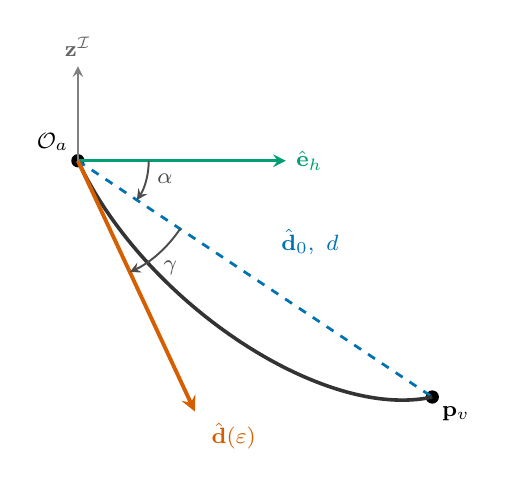
\begin{tikzpicture}[
        >=stealth,
        scale=1.2,
        every node/.style={font=\small},
        chordLine/.style={dashed, okiBlue, line width=1.0pt},
        horizLine/.style={->, okiGreen, line width=1.0pt},
        tetherCurve/.style={black!80, line width=1.3pt},
        tangentVec/.style={->, okiVermillion, line width=1.4pt},
        angleArc/.style={->, line width=0.7pt, black!70}
    ]
        \coordinate (Oa) at (0,0);
        \fill[black] (Oa) circle (2.0pt);
        \node[above left, font=\footnotesize] at (Oa) {$\mathcal{O}_a$};

        \coordinate (Pv) at (3.75,-2.5);
        \fill[black] (Pv) circle (2.0pt);
        \node[below right, font=\footnotesize] at (Pv) {$\mathbf{p}_v$};

        % Local horizontal e_h, within the catenary plane, orthogonal to z^I
        \draw[horizLine] (Oa) -- (2.2,0) node[right, okiGreen, font=\footnotesize] {$\hat{\mathbf{e}}_h$};

        % Chord: taut direction d_0, dashed
        \draw[chordLine] (Oa) -- (Pv);
        \node[above right, okiBlue, font=\footnotesize] at (2.05, -1.1) {$\hat{\mathbf{d}}_0,\ d$};

        % Depression angle alpha, between e_h and the chord
        \draw[angleArc] (Oa) ++(0:0.75) arc (0:-33.69:0.75);
        \node[font=\footnotesize, black!70] at (0.92,-0.19) {$\alpha$};

        % Actual catenary curve
        \draw[tetherCurve] (Oa) .. controls (0.701,-1.503) and (2.604,-2.755) .. (Pv);

        % Tangent (actual tension) direction at O_a
        \draw[tangentVec] (Oa) -- (1.238,-2.654)
            node[below right, okiVermillion, font=\footnotesize, xshift=2pt] {$\hat{\mathbf{d}}(\varepsilon)$};

        % Angle gamma between the chord and the tangent, drawn further out
        \draw[angleArc] (Oa) ++(-33.69:1.3) arc (-33.69:-65:1.3);
        \node[font=\footnotesize, black!70] at (0.977,-1.139) {$\gamma$};

        % Vertical reference at O_a, i.e. z^I, added back since alpha and gamma
        % are now explicitly measured towards it
        \draw[->, black!50, line width=0.7pt] (Oa) -- (0,1.0) node[above, black!60, font=\footnotesize] {$\mathbf{z}^{\mathcal{I}}$};

    \end{tikzpicture}
    \caption{Tether catenary plane.}
    \label{fig:uav_tether_plane}
\end{figure}


The tension direction at $\mathcal{O}_a$ then follows by tilting $\hat{\mathbf{d}}_0$ further towards the vertical by the angle $\gamma(\varepsilon)$, within the same plane,
\begin{equation}
    \hat{\mathbf{d}}(\varepsilon) = \cos\big(\alpha+\gamma(\varepsilon)\big)\,\hat{\mathbf{e}}_h - \sin\big(\alpha+\gamma(\varepsilon)\big)\,\mathbf{z}^{\mathcal{I}},
    \label{eq:uav_tether_direction}
\end{equation}
and the resulting tether force, applied at $\mathcal{O}_a$ and expressed in $\{\mathcal{I}\}$, is
\begin{equation}
    \mathbf{F}_{\mathrm{tether}}^{\mathcal{I}} = T_{\mathrm{tether}}(\varepsilon)\,\hat{\mathbf{d}}(\varepsilon),
    \label{eq:uav_tether_force}
\end{equation}
with $\varepsilon$ evaluated at each instant from \eqref{eq:uav_tether_geometry}--\eqref{eq:uav_tether_slack}. Equation~\eqref{eq:uav_tether_force} is the term $\mathbf{F}_{\mathrm{tether}}^{\mathcal{I}}$ introduced in \eqref{eq:uav_newton}.
